\documentclass[
    DIV12,
    %cleardouble=plain,
    headings=normal,
    pdftex,
    %headexclude,footexclude,
    final,
    bibliography=totocnumbered
    %draft
]{scrreprt}

\usepackage{spreadtab}
\usepackage{xspace}
\usepackage[ngerman]{babel}
\usepackage[utf8]{inputenc}
\usepackage[T1]{fontenc}
\usepackage[pdftex]{graphicx}
\usepackage[bookmarks]{hyperref}
\usepackage{scrpage2}
\usepackage{longtable}
\usepackage{caption, booktabs}
\usepackage{pgf}
\usepackage{float}
\usepackage{xcolor}
\usepackage{colortbl}
\usepackage{relsize}
\usepackage{fancyvrb}
\usepackage{pdfpages} 
\usepackage{multirow}
\usepackage{tabularx}
\usepackage{geometry}
\usepackage{multicol}
\usepackage{multido}
\usepackage{listings}
%\usepackage{hyperref}
\usepackage[autostyle]{csquotes}
\usepackage{eurosym}
\usepackage{subfigure}

\lstset{breaklines=true,
breakatwhitespace = true,
postbreak=\raisebox{0ex}[0ex][0ex]{\ensuremath{\color{red}\hookrightarrow\space}},
escapechar=\^
%literate={\_}{}{0\discretionary{\_}{}{\_}}%
}

%clearpage


\usepackage[
	backend=biber,       % Sortier-Compiler
    style=verbose-trad2, % Zitationsstil   
   sorting=nyt,        % Sortiervorschrift
   abbreviate=false,   % Abkürzungen
   % block=ragged        % Flattersatz
       ]{biblatex}
\bibliography{mybib}
\bibstyle{IEEEtran}

\newcommand{\tabitem}{~~\llap{\textbullet}~~}

\graphicspath{{./}{./images/}{./chapter/images/}}

 

% #################################################################

%\hyphenation{Cha-otn-gsch-werl}
%\setlength\headheight{1.75cm}

%\ihead{\includegraphics[height=0.05\textheight]{HS_Hof_Logo}}
\chead{}
%\ohead{\includegraphics[height=0.05\textheight]{audi_logo}}
\pagestyle{scrheadings}

\setcounter{secnumdepth}{3}
\setcounter{tocdepth}{3}
\renewcommand{\arraystretch}{1}

%\parskip0.5\baselineskip plus 0.125\baselineskip minus 0.25\baselineskip
\parindent0em

% #################################################################

%\def\SECH{S\kern-.075em \lower.5ex\hbox{E}\kern-0.05em CH\xspace}
%\def\SEARCH{S\kern-.075em \lower.5ex\hbox{E}\kern-0.05em AR\kern-.075em \raise.5ex\hbox{C}\kern-0.05em H\xspace}

% #################################################################

% ########Farbanpassung HS Hof #########
\definecolor{HSHofgrey}{HTML}{646466}

\addtokomafont{chapter}{\color{HSHofgrey}}
\addtokomafont{section}{\color{HSHofgrey}}
\addtokomafont{caption}{\color{HSHofgrey}}
\addtokomafont{subsection}{\color{HSHofgrey}}
\addtokomafont{subsubsection}{\color{HSHofgrey}}
\setkomafont{captionlabel}{\color{HSHofgrey}}




\automark[section]{chapter}
%%\titlehead{{ \hfill \includegraphics[width = 0.5\textwidth]{HS_Hof_Logo} \hfill
%%\includegraphics[width = 0.4\textwidth]{audi_logo}}
%\hfill
%}
\subject{Semesterprojekt}
\title{Entwicklung eines Concierge- Behaviours für den humanoiden Roboter Pepper}
%\subtitle{\Large zur Erlangung des akademischen Grades \\
%Bachelor of Science}
\author{vorgelegt von \\ \textbf{Julian Keller, Eric Meiß, Caroline Fichtner, Lothar Mödl}}
\date{
\begin{tabular}{rl}
\textbf{Studiengang:} & Mobile Systeme \\\textbf{Fakultät:} & Informatik \\
\end{tabular}
}
\publishers{\vfill
	\begin{tabular}{rl}
\textbf{Ausgabetermin}: & 12.10.2017  \\	
\textbf{Abgabetermin}:  & 24.01.2018 \\	
%   & \\	
\textbf{Erstprüfer}:    & Prof. Dr. Elmar Cochlovius \\	
%\textbf{Zweitprüfer}:  & Prof. Dr. Michael Stepping\\	
%\textbf{Betreuer}: & Junhao Chen\\
	\end{tabular}}


%\author{Lothar Mödl}
%\date{Version 0.0.1}

% #################################################################

\begin{document}
\flushbottom
\lstdefinelanguage{swift}
{
  morekeywords={
    func,if,then,else,for,in,while,do,switch,case,default,where,break,continue,fallthrough,return,
    typealias,struct,class,enum,protocol,var,func,let,get,set,willSet,didSet,inout,init,deinit,extension,
    subscript,prefix,operator,infix,postfix,precedence,associativity,left,right,none,convenience,dynamic,
    final,lazy,mutating,nonmutating,optional,override,required,static,unowned,safe,weak,internal,
    private,public,is,as,self,unsafe,dynamicType,true,false,nil,Type,Protocol,
  },
  morecomment=[l]{//}, % l is for line comment
  morecomment=[s]{/*}{*/}, % s is for start and end delimiter
  morestring=[b]" % defines that strings are enclosed in double quotes
}

\definecolor{keyword}{HTML}{BA2CA3}
\definecolor{string}{HTML}{D12F1B}
\definecolor{comment}{HTML}{008400}

\lstset{
  language=swift,
  basicstyle=\ttfamily,
  showstringspaces=false, % lets spaces in strings appear as real spaces
  columns=fixed,
  keepspaces=true,
  keywordstyle=\color{keyword},
  stringstyle=\color{string},
  commentstyle=\color{comment},
}

\maketitle

\pagenumbering{arabic}
\tableofcontents
% Kapitel 1
		\setcounter{page}{1}
		\pagenumbering{arabic}


\chapter{Einführung}
\section{Zielsetzung}
//Hier kommen unsere Ziele hin

\section{Motivation}
//Hier kommt hin, warum wir das Projekt machen


\section{Ziele der Arbeit}
\label{Ziele}
//Evtl. nochmal stichpunktartig die konkreten Ziele auflisten







				\cleardoublepage	

			% Kapitel 2
			
\chapter{Allgemeine Grundlagen}
\label{chap:Allgemeine Grundlagen} 
//Hier allgemeine Begriffe klären bzw. Grundlagen für die weitere Verwendung schaffen



\section{Projektorganisation und Dokumentation}
//Evtl. erklären, welche Tools wir verwendet haben etc.
			
				\cleardoublepage	
			% Kapitel 3
			\chapter{Funktionsmodell}
Dieses Kapitel beschreibt die allgemeine Idee, sowie die theoretischen Funktionen der Anwendung.

//In diesem Kapitel werden alle Funktionen, die wir umsetzen wollen, beschrieben, inkl. Use-Case-Diagramme

\section{Begrüßung der Personen}


\section{Roomtour}

\subsection{Empfangsbereich}

\subsection{Schlafzimmer}

\subsection{Wohnzimmer}

\subsection{Küche}

\section{Lichtsteuerung}

\section{Fenstersteuerung}
				\cleardoublepage
			% Kapitel 4
			\chapter{Datenmodell}

//Hier wird die Datenstruktur des Projekts beschrieben
				\cleardoublepage
			\chapter{Funktionalitäten}

//Erklärung aller Funktionalitäten (aus der Spezifikation) auf technischer Ebene, d.h. mit Sequenzdiagrammen inkl. genauer Methodenbeschreibung

			
			\cleardoublepage
			\chapter{Klassendiagramme}

\section{Übersicht Klassendiagramm}

\section{Übersicht der Methoden der Klassen}
			
			\cleardoublepage
			\chapter{Framework}
//Evtl. Beschreibung eigen erstellter Frameworks und deren Verwendung
		
			\cleardoublepage
			\chapter{Erfüllung der Ziele}

//Evtl. Beschreibung der erfüllten/nicht erfüllten Ziele (von Anfang der Arbeit) 


\chapter{Ausblick}

//Ausblick/Schluss
			%\cleardoublepage
			\printbibliography
			%\appendix
\chapter{Realisierung des Prototypen}

\begin{figure}[ht]
	\centering
	\subfigure[Prototyp - Übersicht aller Außenlichtoptionen]{\includegraphics[width=0.49\textwidth]{SS_Overview}}
	\subfigure[Prototyp - Detailansicht einer Außenlichtoption]{\includegraphics[width=0.49\textwidth]{SS_Detail}}
	\caption{Prototyp: Übersicht der Lichtoptionen und Detailansicht}
\end{figure}

\begin{figure}[ht]
	\centering
	\subfigure[Prototyp - Kauf einer Außenlichtoption mit Apple Pay]{\includegraphics[width=0.49\textwidth]{SS_ApplePay}}
	\subfigure[Prototyp - Übersicht aller Credits-Pakete]{\includegraphics[width=0.49\textwidth]{SS_Credits}}
	\caption{Prototyp: Kauf einer Lichtoption und eines Credits-Paktes}
\end{figure}

\begin{figure}[ht]
	\centering
	\subfigure[Prototyp - Auswahl der Währung beim Kauf]{\includegraphics[width=0.49\textwidth]{SS_Buy}}
	\subfigure[Prototyp - Auswahl der Währung beim Abonnieren]{\includegraphics[width=0.49\textwidth]{SS_Subscription}}
	\caption{Prototyp: Auswahl der Währung}
\end{figure}

\chapter{Klassendiagramme}
\label{appendix:KD}
\begin{figure}[ht]
	\centering
		\subfigure[Klassendiagramm: DatabaseController]{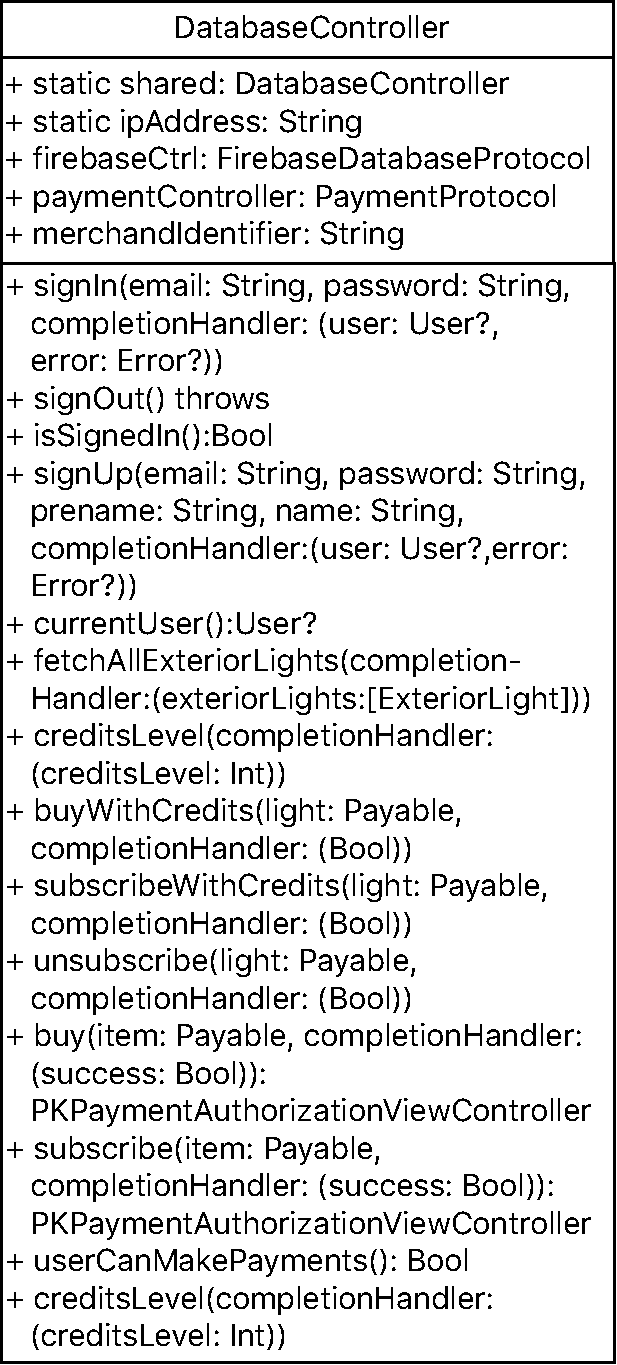
\includegraphics[width=0.45\textwidth]{KD_DatabaseController}}
	\subfigure[Klassendiagramm: ApplePayButton]{\includegraphics[width=0.45\textwidth]{KD_ApplePayButton}}
	\caption{Klassendiagramme: DatabaseProtocol und ApplePayButton}
	\label{appendix:KD:DatabaseCtrlApplePay}
\end{figure}


\begin{figure}[ht]
	\centering
	\subfigure[Klassendiagramm: CreditsPaymentProtocol]{\includegraphics[width=0.47\textwidth]{KD_CreditsPayment}}
		\subfigure[Klassendiagramm: CreditsPackage]{\includegraphics[width=0.49\textwidth]{KD_CreditsPackage}}
	\caption{Klassendiagramme: CreditsPaymentProtocol und CreditsPackage}
	\label{appendix:KD:CreditsPaymentCreditsPackage}
\end{figure}


\begin{figure}[ht]
	\centering
		\subfigure[Klassendiagramm: ExteriorLight]{\includegraphics[width=0.49\textwidth]{KD_ExteriorLight}}
		\subfigure[Klassendiagramm: PaymentController]{\includegraphics[width=0.49\textwidth]{KD_PaymentController}}
	\caption{Klassendiagramme: ExteriorLight und PaymentController}
	\label{appendix:KD:ExteriorLightPaymentController}
\end{figure}


\begin{figure}[ht]
	\centering
	\subfigure[Klassendiagramm: FirebaseDatabaseController]{\includegraphics[width=0.49\textwidth]{KD_FirebaseDatabaseController}}
	\subfigure[Klassendiagramm: LightProtocol]{\includegraphics[width=0.49\textwidth]{KD_LightProtocol}}
	\caption{Klassendiagramme: FirebaseDatabaseController und LightProtocol}
	\label{appendix:KD:FirebaseDatabaseCtrlLightProtocol}
\end{figure}

\begin{figure}[ht]
	\centering
	\subfigure[Klassendiagramm: MoneyPaymentProtocol]{\includegraphics[width=0.49\textwidth]{KD_MoneyPaymentProtocol}}
	\subfigure[Klassendiagramm: PKPaymentAuthorizationViewControllerDelegate]{\includegraphics[width=0.49\textwidth]{KD_PKPaymentAuthorizationViewControllerDelegate}}
	\caption{Klassendiagramme: MoneyPaymentProtocol und PKPaymentAuthorizationViewControllerDelegate}
	\label{appendix:KD:MoneyPaymentPKPayment}
\end{figure}

\begin{figure}[ht]
	\centering
		\subfigure[Klassendiagramm: PaymentProtocol]{\includegraphics[width=0.49\textwidth]{KD_PaymentProtocol}}
	\subfigure[Klassendiagramm: DecodeableProtocol]{\includegraphics[width=0.49\textwidth]{KD_DecodeableProtocol}}
	\caption{Klassendiagramme: PaymentProtocol und DecodeableProtocol}
	\label{appendix:KD:PaymentProtocolDecodeableProtocol}
\end{figure}

\begin{figure}[ht]
	\centering
			\subfigure[Klassendiagramm: User]{\includegraphics[width=0.47\textwidth]{KD_User}}
\subfigure[Klassendiagramm: PackageProtocol]{\includegraphics[width=0.47\textwidth]{KD_PackageProtocol}}
	\caption{Klassendiagramme: User und PackageProtocol}
	\label{appendix:KD:UserPackageProtocol}
\end{figure}



	

			% Literaturverzeichnis
			% \nocite{*}
			

\listoffigures

\end{document}
